\documentclass[tikz,border=10pt]{standalone}
\begin{document}
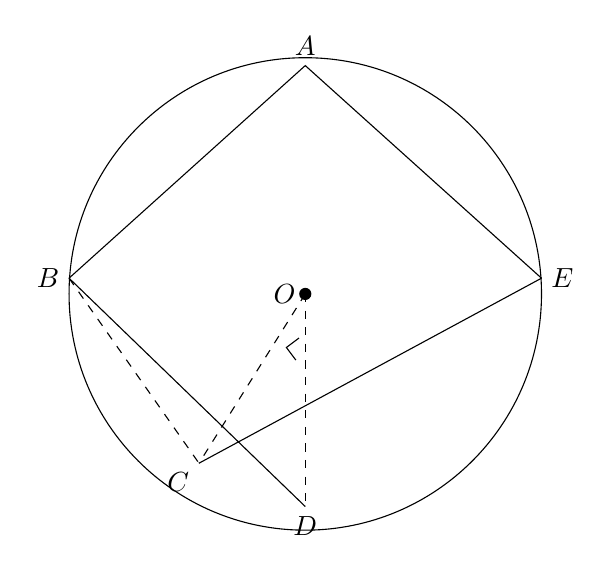
\begin{tikzpicture}[scale=1]

% Coordinates
\coordinate (O) at (0,0);
\coordinate (A) at (0,2.9);
\coordinate (B) at (-3.0,0.2);
\coordinate (E) at (3.0,0.2);
\coordinate (D) at (0,-2.7);
\coordinate (C) at (-1.35,-2.15);

% Circle
\draw (O) circle [radius=3];

% Solid polygon/chords
\draw (B) -- (A) -- (E);
\draw (B) -- (D);
\draw (C) -- (E);

% Dashed segments
\draw[dashed] (B) -- (C);
\draw[dashed] (O) -- (C);
\draw[dashed] (O) -- (D);

% Right-angle mark at O between OC and OD
\draw (-0.08,-0.56) -- (-0.24,-0.68) -- (-0.12,-0.84);

% Point O
\fill (O) circle (2.2pt);

% Labels
\node[above] at (A) {$A$};
\node[left] at (B) {$B$};
\node[right] at (E) {$E$};
\node[below] at (D) {$D$};
\node[below left] at (C) {$C$};
\node[left] at (O) {$O$};

\end{tikzpicture}
\end{document}
